\documentclass[11pt]{article}
\usepackage[margin=0.8in]{geometry}
\usepackage{fontspec}
\setmainfont{Avenir Next}
\setsansfont{Avenir Next}
\usepackage{booktabs}
\usepackage{graphicx}
\usepackage{xcolor}
\usepackage{hyperref}
\usepackage{microtype}
\usepackage{enumitem}
\usepackage{fancyhdr}
\definecolor{navy}{HTML}{15324A}
\definecolor{muted}{HTML}{536471}
\definecolor{panel}{HTML}{F2F6F8}
\hypersetup{colorlinks=true,linkcolor=navy,urlcolor=navy}
\pagestyle{fancy}
\fancyhf{}
\lhead{\small Shared-state activity poll}
\rhead{\small \thepage}
\renewcommand{\headrulewidth}{0.3pt}
\setlength{\parindent}{0pt}
\setlength{\parskip}{0.6em}
\setlist{nosep,leftmargin=1.4em}

\begin{document}

{\color{navy}\LARGE\bfseries Path Dependence in a Shared-State Activity Poll}

\vspace{0.4em}
{\Large Ten repeated EDSL simulations with sequentially visible votes}

\vspace{1.2em}
\colorbox{panel}{\parbox{0.94\linewidth}{
\textbf{Main result.} The same balanced preference distribution produced four different
winners. Winner frequency was bike ride: 3, sailing: 3, hike: 3, beach day: 1. Once an early lead formed,
later agents' desire to join the group often amplified it into a large majority.
}}

\section*{Research question}

Can sequentially visible choices produce different collective outcomes when the group's
underlying activity preferences begin balanced? This demonstration repeats the same
shared-state survey ten times. It is designed to make the mechanism observable: every
agent reads the current vote register, answers once, and writes one vote.

\section*{Experimental design}

Each run contains 16 simulated participants and four activities: \textit{bike ride},
\textit{sailing}, \textit{hike}, and \textit{beach day}. Exactly four participants
prefer each activity before ordering. Each participant also receives:

\begin{itemize}
  \item a preference strength drawn from 0.60 to 0.90; and
  \item a conformity value drawn from 0.55 to 0.90.
\end{itemize}

The ordering and trait values vary with the run seed. Agents are prompted through
Gemini 2.5 Flash using local EDSL orchestration. A grouped round-robin schedule creates
an ordering barrier, so voter $t$ sees the state committed by voters $1,\ldots,t-1$.
Across the ten runs there are 160 decisions.

\section*{Shared-state mechanism}

For each participant, the survey executes the following sequence:

\begin{center}
\fbox{\parbox{0.84\linewidth}{
\textbf{1. Read} the vote register at version $t-1$ $\rightarrow$
\textbf{2. Ask} the activity question with that snapshot $\rightarrow$
\textbf{3. Write} the selected activity $\rightarrow$
\textbf{4. Commit} version $t$.
}}
\end{center}

The explicit read is important. It records what the participant could observe and makes
the prompt's state dependency auditable in the Results provenance. Concurrency limits
alone would not create this sequence; the schedule supplies the barrier between turns.

\clearpage
\section*{Outcomes across repetitions}

\begin{center}
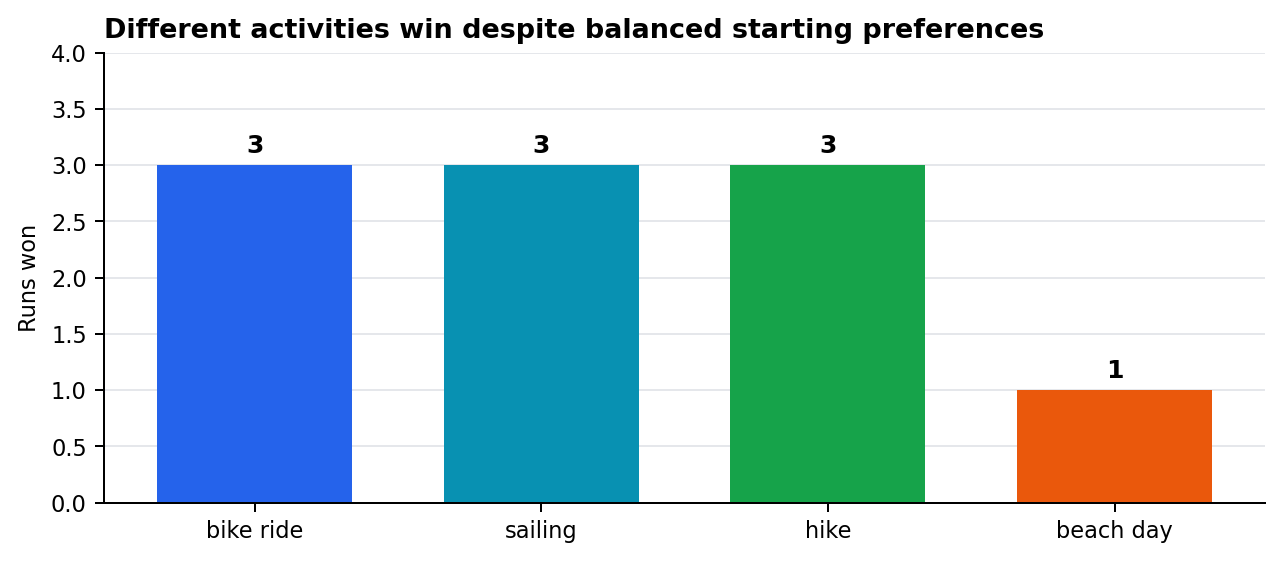
\includegraphics[width=0.78\linewidth]{winner_frequency.png}
\end{center}

The mean winning total was 12.9 of 16 votes. Participants selected
their initially preferred activity in 44.4% of decisions; the remaining
choices provide a direct descriptive measure of departures from baseline preference.

\begin{center}
\centering
\footnotesize
\resizebox{\linewidth}{!}{%
\begin{tabular}{r p{3.0cm} rrrr l}
\toprule
Run & First three votes & Bike & Sail & Hike & Beach & Winner \\
\midrule
1 & beach day, hike, sailing & 1 & 9 & 3 & 3 & sailing \\
2 & hike, hike, sailing & 3 & 4 & 5 & 4 & hike \\
3 & bike ride, bike ride, bike ride & 16 & 0 & 0 & 0 & bike ride \\
4 & sailing, beach day, sailing & 0 & 15 & 0 & 1 & sailing \\
5 & sailing, sailing, sailing & 1 & 14 & 1 & 0 & sailing \\
6 & bike ride, sailing, beach day & 2 & 2 & 3 & 9 & beach day \\
7 & hike, hike, hike & 0 & 1 & 15 & 0 & hike \\
8 & hike, sailing, hike & 0 & 1 & 15 & 0 & hike \\
9 & bike ride, bike ride, bike ride & 16 & 0 & 0 & 0 & bike ride \\
10 & bike ride, bike ride, bike ride & 15 & 0 & 0 & 1 & bike ride \\
\bottomrule
\end{tabular}
}

\smallskip
{\small\textbf{Table 1.} Final counts and the earliest observed path. Preferences were balanced 4--4--4--4 in every run.}
\end{center}

\clearpage
\section*{How the vote paths evolved}

\begin{center}
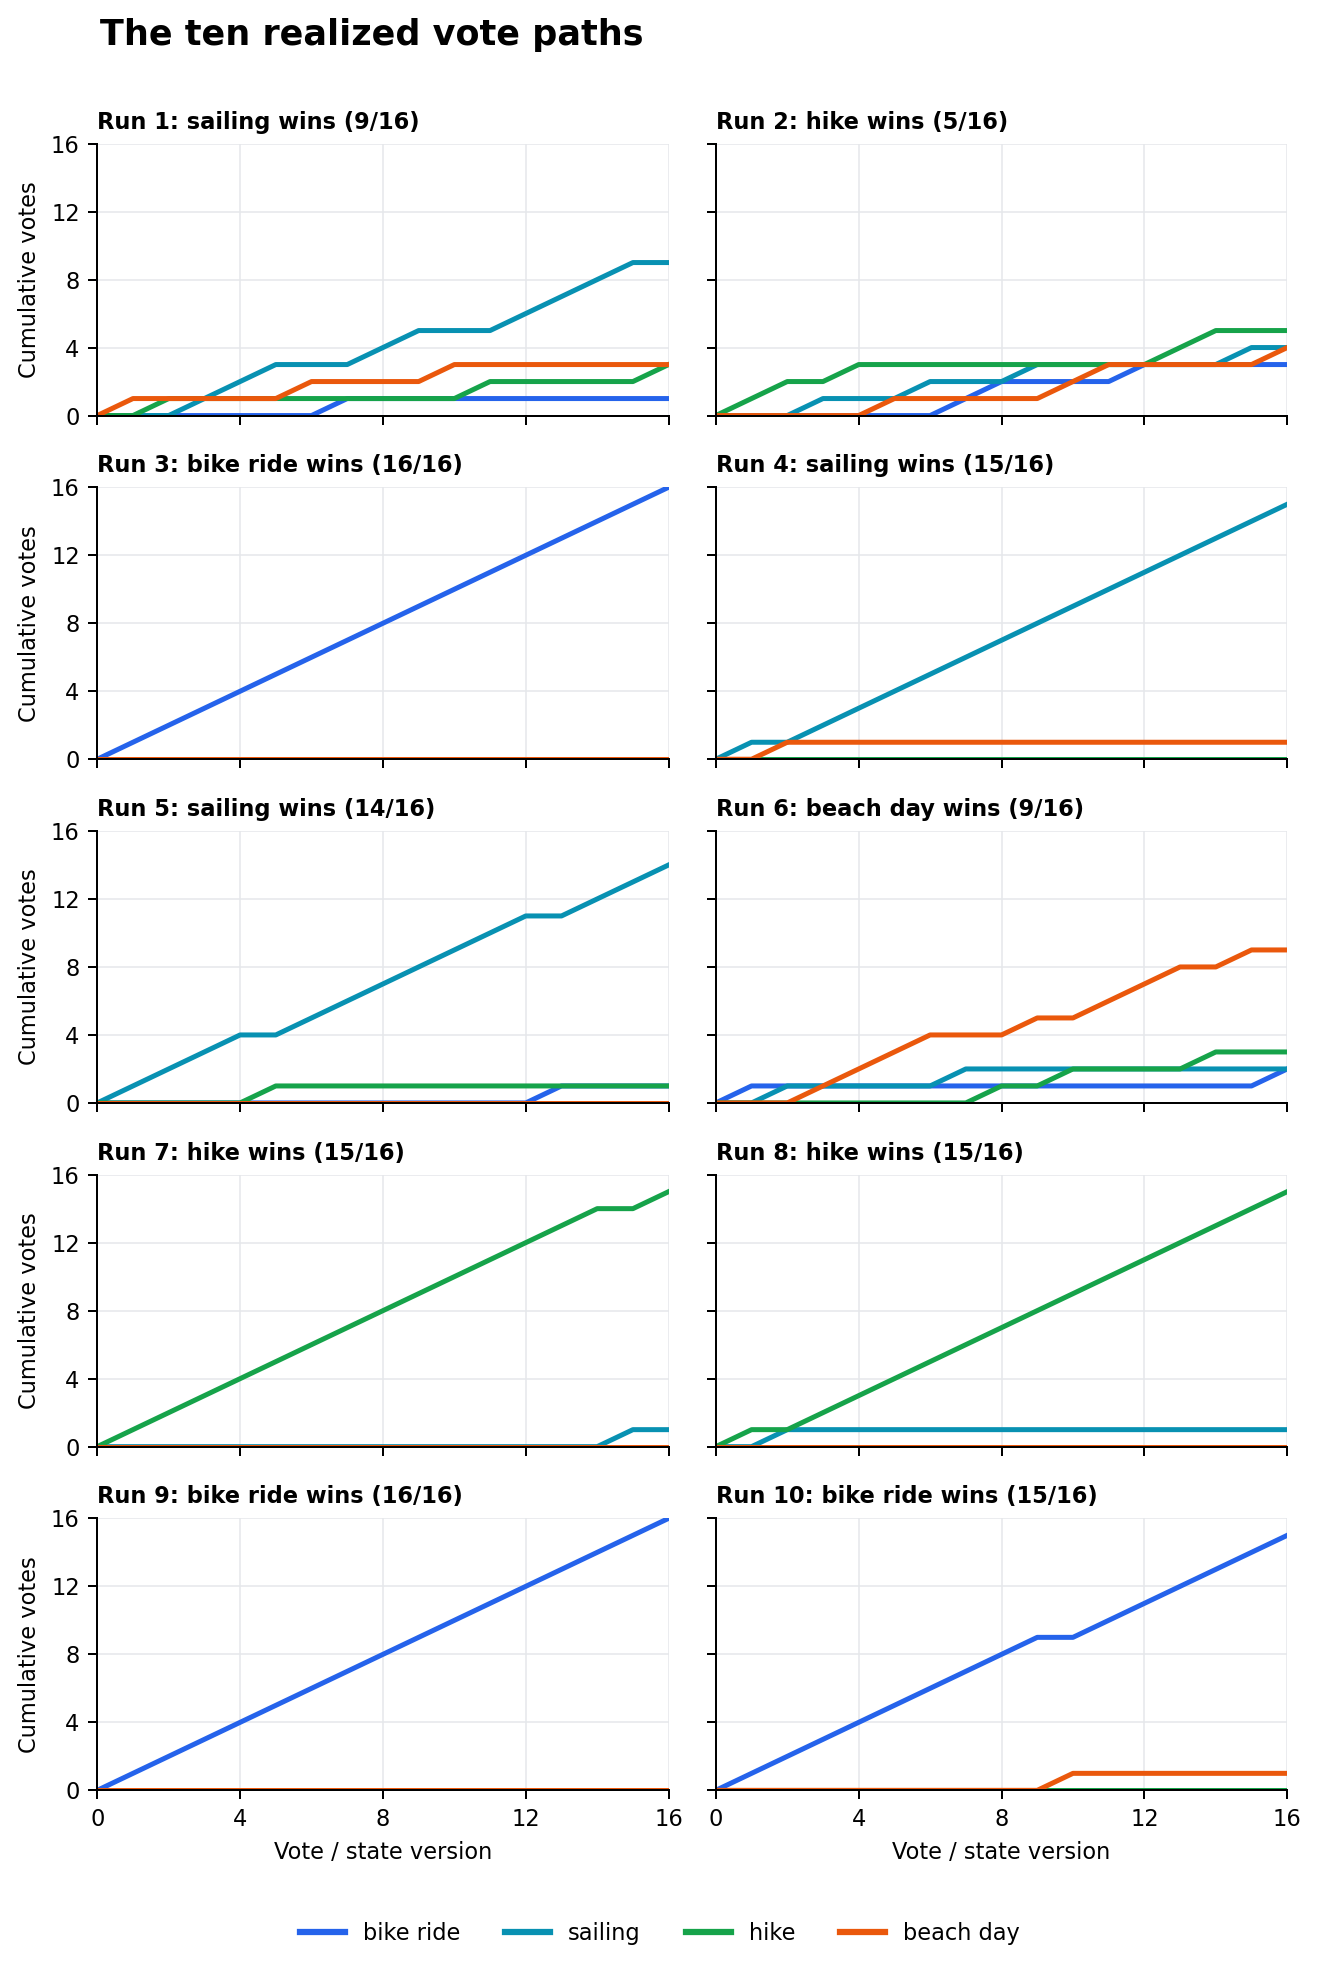
\includegraphics[height=0.84\textheight]{vote_paths.png}
\end{center}

\clearpage
\section*{What the repetitions show}

\textbf{Multiple outcomes occurred.} Bike ride, sailing, hike, and beach day each won
at least once, even though every run began with four agents assigned to prefer each
activity.

\textbf{Early positions were informative.} The eventual winner was among the activity
or activities tied for the lead after three votes in 10 of 10 runs.
This wording matters: runs with three different opening votes have a three-way early tie,
not a unique predictor.

\textbf{Some paths cascaded.} Runs 3 and 9 ended 16--0; runs 4, 7, 8, and 10 ended
15--1. The line plots expose when those gaps opened and whether later voters reinforced
them.

\textbf{Interpretation.} The simulations are consistent with a path-dependent process:
early random variation changes the public state, and the public state can influence later
choices. They do not, by themselves, estimate a causal conformity effect. Both the trait
draws and model sampling vary across runs.

\section*{Limitations and next tests}

\begin{itemize}
  \item Ten repetitions are illustrative rather than a stable estimate of outcome probabilities.
  \item The agents are language-model simulations, not human participants.
  \item Ordering, trait values, and model stochasticity vary together in this version.
  \item A stronger test would hold personas fixed, randomly permute only their order, and run many more repetitions.
  \item A no-visibility control would separate preference-driven choices from responses to the live vote register.
\end{itemize}

\section*{Reproducibility}

The report is generated from
\nolinkurl{shared-state-activity-poll-repeated.json}. The single-run implementation is
\nolinkurl{shared_state_activity_poll.py}, the ten-run driver is
\nolinkurl{shared_state_activity_poll_repeated.py}, and the report builder is
\nolinkurl{build_shared_state_path_dependence_report.py}.

\vfill
{\small\color{muted} Generated from the saved event-level output on 30 August 2026.}

\end{document}
